\documentclass[entwurf.tex]{subfiles}

\begin{document}
\chapter{Klassendiagramme}
	\section{Bus}
		
  		In diesem Diagramm ist der Aufbau des Moduls ''Bus'' zu sehen. Die Kommunikation aller Module ist entkoppelt und findet größtenteils über den Austausch von Nachrichten verschiedener Typen über den Bus statt. Um mit dem Bus arbeiten zu können, muss ein Modul eine Klasse besitzen, die von ''BusDevice'' erbt. Der Bus funktioniert als eine Variation des Beobachter-Entwurfsmusters. Eine von ''BusDevice'' erbende Klasse kann über subscribe() bzw. unsubscribe() auf dem ''MessageBus'' Nachrichten eines bestimmten Topics (Sensortyp, Datenbanknachrichten, Konfigurationsnachrichten) abonnieren. \\
  		Diese Abbonements werden in der Klasse ''Broker'' verwaltet. Sendet ein Objekt von ''BusDevice'' über publish() eine Nachricht an ''MessageBus'', so holt sich letzterer von seinem Broker eine Liste über alle Abonnements für das Topic der Nachricht und sendet diese dann an alle abonnierenden Objekte. Das versenden einer Nachricht sowie deren Empfang sind asynchrone Funktionsaufrufe. \\
  		Die Oberklasse ''Message'' besitzt eine Reihe von erbenden Klassen. Dies ist nötig, um alle möglichen Typen von Nachrichten darzustellen: ''SensorValueMessage'' wird für das einfache versenden von Messwerten benutzt, ''ConfigFileRequest'' für Konfigurationsdateien usw. Dieser Aufbau ermöglicht das leichte Ergänzen um ggf. zusätzlich benötigte Nachrichtentypen. Ein besonderer Nachrichtentyp ist die DatabaseRequestMessage, die Anfragen an die Datenbank beinhaltet. Die Anfragen vom Typ ''DBRequest'' sind unterteilt in verschiedene Typen von Anfragen: DBReqRecent fordert die letzten n Einträge an, DBReqFrom alle Einträge seit einem Datum, und DBReqRange fordert alle Datenbankeinträge zwischen zwei Daten an. \\
  		Das Konstrukt  der Klassen ''BusDevice'' sowie erbende Klassen, ''Message'' und die von ''Message'' erbenden Klassen ergeben gemeinsam das Entwurfsmuster der Fabrikmethode. 
  		
  		\begin{figure}[H]
  			\begin{center}
 				\makebox[\textwidth][c]{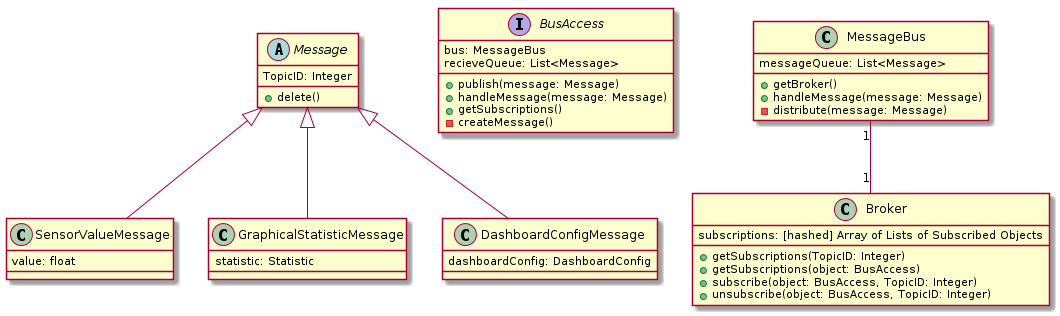
\includegraphics[width=0.8\paperheight, angle=90]{diagrams/Bus.png}}
  				\caption{Bus Klassendiagramm}
  			\end{center}
  		\end{figure}
  	
  	\newpage
  	\section{Virtual Sensors}
		Hier sieht man den Aufbau der Virtuellen Sensoren.
		\begin{figure}[H]
  			\begin{center}
 				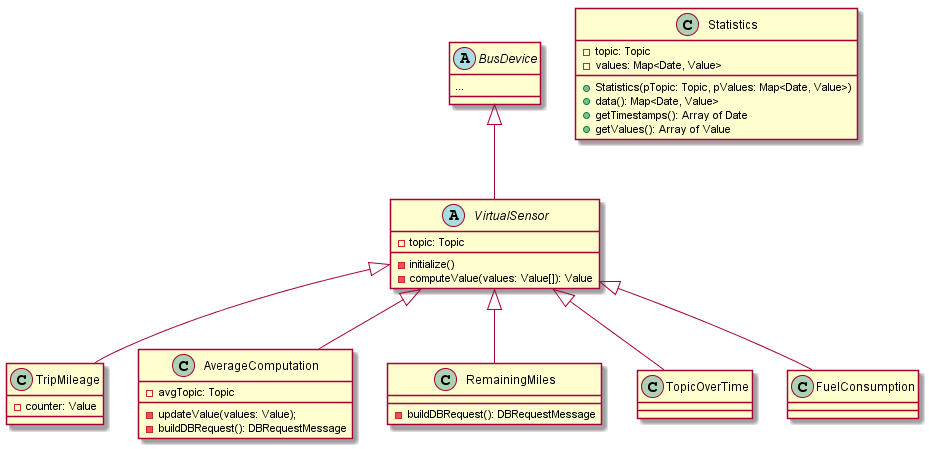
\includegraphics[width=0.8\textheight,angle=90]{diagrams/VirtualSensors.png}
  				\caption{Virtuelle Sensoren Klassendiagramm}
  			\end{center}
  		\end{figure}
  	\newpage
  	\section{Database Access}
  		Im folgenden Diagramm ist der Aufbau der Datenbank und des Datenbankzugriffs zu sehen.
  		\begin{figure}[H]
  			\begin{center}
 				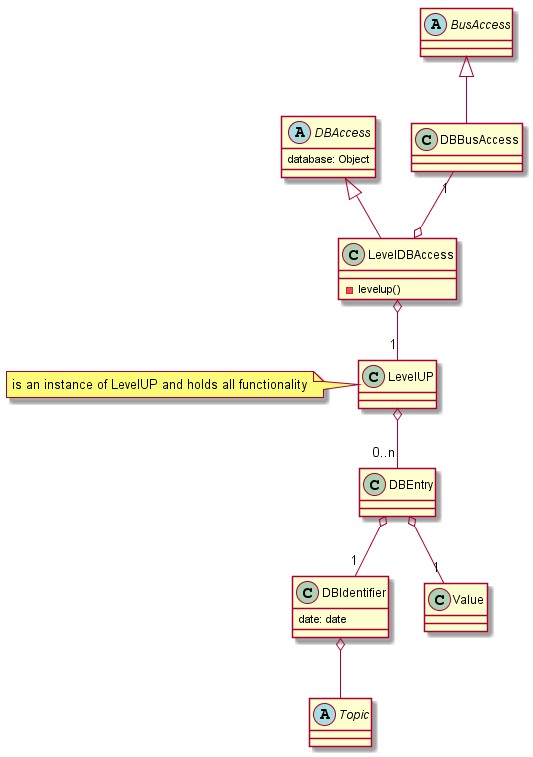
\includegraphics[width=0.8\textwidth]{diagrams/DBAccess.png}
  				\caption{Virtuelle Sensoren Klassendiagramm}
  			\end{center}
  		\end{figure}
  	Als Datenbank wurde, wie im Pflichtenheft spezifiziert, LevelDB benutzt. Die Access-Klasse für LevelDB erbt von einer ''DBAccess''-Oberklasse, um leichte Austauschbarkeit zu gewährleisten. In der LevelDBAccess-Klasse wird außer der Referenz auf die LevelUp-Instanz auch der aktuelle Fahrer sowie die spezifizierte maximale Kapazität der Datenbank gehalten. \\ In der Datenbank, im Fall von LevelDB ein einfacher Key-Value-Store, werden zwei Typen von Objekten gehalten: Zum einen werden mit der Zeit und dem Typ des Sensors als Key Objekte von Sensorwerten und Fahrer gespeichert, zum anderen fahrerbezogene Einträge, die präferierten Kraftstoff und eine Referenz auf die Konfiguration des virtuellen Armaturenbretts mit der Identifikation des Fahrers als Key gespeichert werden. Zur Kommunikation mit anderen Modulen besitzt der Datenbankzugriff mit DBBusDevice eine Klasse, die den Zugang zum Bus möglich macht und Nachrichten vom Bus dekodiert. 
  	

	\newpage
  	\section{Website}
  	\label{Class:Website}
		Hier ist zu sehen wie die Seite allgemein aufgebaut ist. Die Website besteht aus zwei Frames. In einem wird die Statusbar angezeigt, im anderen werden können verschiedene Views sichtbar sein. Unter anderem z.B. das GridView auf dem die Dashes angezeigt werden. Für weiteres siehe: \nameref{Class:GridView}, \nameref{Class:SettingsView}.
		
		Die Elemente der Statusbar können unter anderem Text, Knöpfe und Icons sein.
		\begin{figure}[H]
  			\begin{center}
 				\makebox[\textwidth][c]{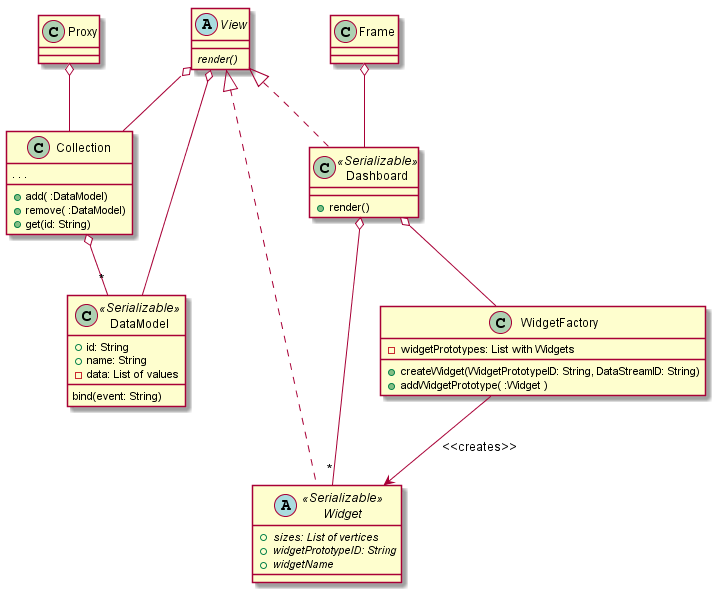
\includegraphics[width=0.8\paperwidth]{diagrams/website.png}}
  				\caption{UI Klassendiagramm}
  			\end{center}
  		\end{figure}  	
  	
  	\newpage
  	\section{User Interface}
		Wie in \ref{Class:Website} zu sehen ist besteht ein Hauptteil des UserInterface aus dem ViewFrame der von verschiedenen Views vertreten werden kann. Hier sieht man den Aufbau des GridViews und des SettingViews. Das Grid nutzt eine Objekt der Klasse Gridster die aus der Bibliothek Gridster stammt. Das GridView besteht hauptsächlich aus diesem Objekt. Es ermöglicht verschiedene Widgets in einem Grid mit Elementen verschiedener Größen dynamisch anzeigen zu lassen.
		
		Hierbei sind die Widgets selbst Abonnenten des angezeigten Signals, weshalb diese die abstrakte Klasse BusDevice implementieren müssen.
		
		Über die SettingsView ist es möglich verschiedene Widgets in dieses Grid hinzuzufügen oder zu ändern. Weshalb sich das SettingView immer die Instanz des Grids als Objekt speichert. Dies kommt zum Einsatz wenn z.B. ein früherer Zustand des Serializable Grids wiederhergestellt werden soll. Um früher gespeicherte Konfigurationen vom Bus zu empfangen und neue Einstellungen an den Server zu schicken implementiert auch die SettingsView den BusDevice. 
		
		
		\begin{figure}[H]
  			\begin{center}
 				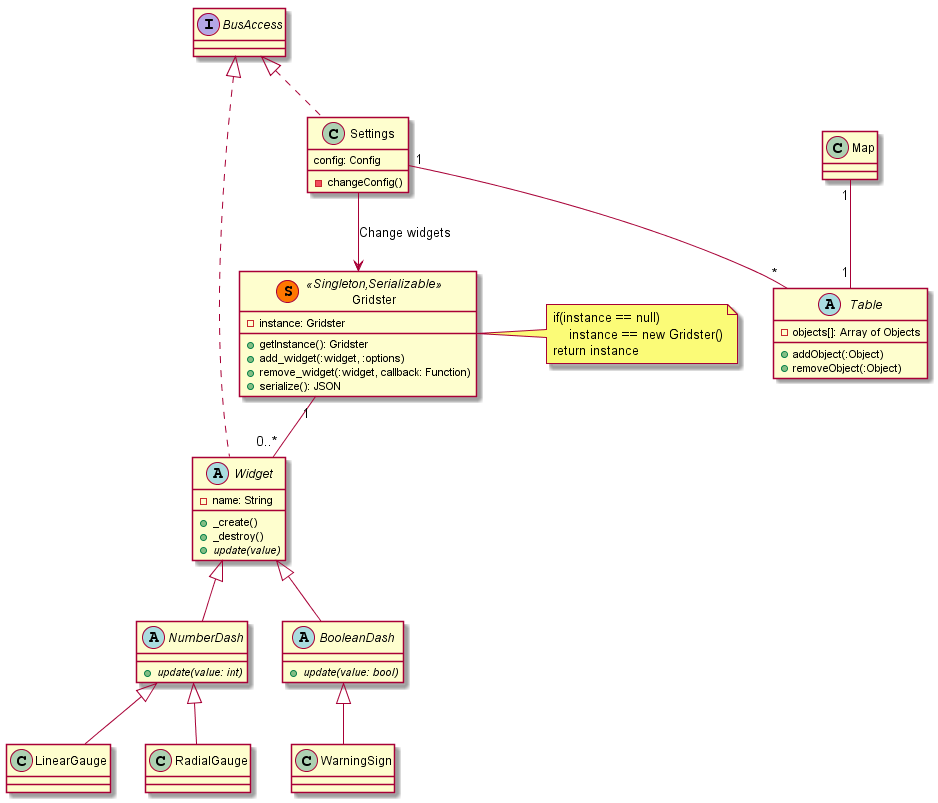
\includegraphics[width=\textwidth]{diagrams/UI.png}
  				\caption{UI Klassendiagramm}
  			\end{center}
  		\end{figure}
  		
  		
  		
  	\newpage
  	\section{Parking Sensor Serverside}
		Hier ist zu sehen wie das Rückfahrassistenzsystem aufgebaut ist. Siehe auch %TODO Link sequenzdiagramm
		\begin{figure}[H]
 			\makebox[\textwidth][c]{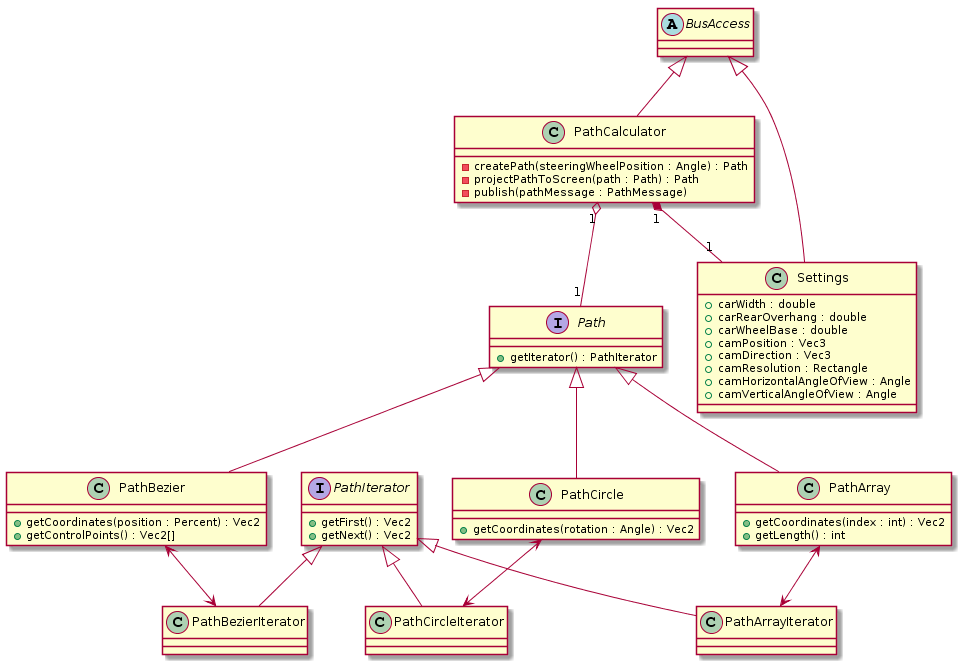
\includegraphics[width=\textwidth]{diagrams/ParkingSensor/v3/classdiagram_server.png}}
  			\caption{Rückfahrsystem Klassendiagramm}
  		\end{figure}
  		
  	\newpage
  	\section{Parking Sensor Clientside}
		Hier ist zu sehen wie das Rückfahrassistenzsystem aufgebaut ist. Siehe auch %TODO Link sequenzdiagramm
		\begin{figure}[H]
 			\makebox[\textwidth][c]{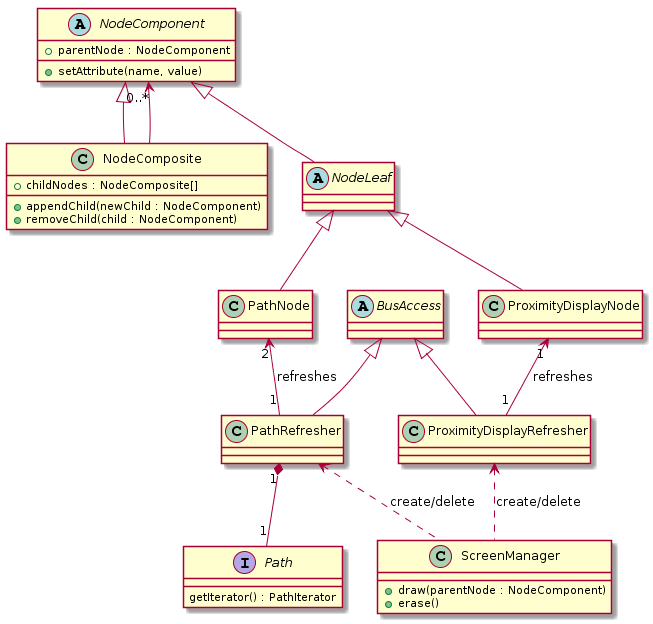
\includegraphics[width=\textwidth]{diagrams/ParkingSensor/v3/classdiagram_userdevice.png}}
  			\caption{Rückfahrsystem Klassendiagramm}
  		\end{figure}
  	
  	
\chapter{Klassen}
	\section{Bus}
	\subsection{BusDevice}
	\label{Class:BusDevice} 
		Eine abstrakte Klasse, deren erbende Klassen Zugriff auf das Bus-Modul haben.
		\begin{description}
			\attr{private messages: List of Messages} 
				Noch zu versendende Nachrichten
			\method{public publish(message: Message): Boolean}
			
				Sendet eine Nachricht asynchron an eine Instanz von MessageBus.\\ 
				\textbf{Parameter:} Die zu versendende Nachricht.\\ 
				\textbf{Rückgabewert:} Boolean, der beschreibt, ob die Nachricht beim Bus angekommen ist.
			\method{abstract public handleMessage(message: Message): Void}  
				Funktion zum asynchronen Empfangen einer Nachricht von einer Instanz von MessageBus.\\ 
			\method{public subscribe(object: BusDevice, topic: Topic): boolean} 
				Funktion zum abonnieren von Nachrichten eines bestimmten Themas.\\ 
				\textbf{Parameter:} Der Abonnent und das abonnierte Thema.\\ 
				\textbf{Rückgabewert:} Boolean, der beschreibt, ob das Thema erfolgreich abonniert wurde.
			\method{public unsubscribe(object: BusDevice, topic: Topic): boolean} 
				Funktion zum Beenden eines Abonnements zu einem bestimmten Thema.\\ 
				\textbf{Parameter:} Der Abonnent und das abonnierte Thema.\\ 
				\textbf{Rückgabewert:} Boolean, der beschreibt, ob das Thema erfolgreich aus der Liste der Abonnements entfernt wurde.
			\method{private createMessage(): Message} 
				Funktion zum Erzeugen einer neuen Nachricht. Die Funktion sollte in den meisten Fällen von der erbenden Klasse überschrieben werden. \\
				\textbf{Rückgabewert}: Die neu erzeugte Nachricht.
		\end{description}
  		
	\subsection{Message}
	\label{Class:Message} 
		Eine abstrakte Klasse, die als Muster für alle Nachrichten dient, die über den Bus versendet werden können.
		\begin{description}
			\attr{protected topic: Topic}  
				Das Thema der Nachricht; wird zur Identifikation des Nachrichtentyps sowie des Inhalts der Nachricht benutzt.
			\attr{Inhalt}
				Der Inhalt der Nachricht, ist je nach erbender Klasse von einem unterschiedlichen Typ.
		\end{description}
	\subsection{MessageBus}
	\label{Class:MessageBus}
		Die Klasse, die die Funktionalität des Busses beinhaltet.
		\begin{description}
			\attr{private broker: Broker}
				Der Broker des Busses; siehe Beschreibung der Broker-Klasse. \\
				
			\method{public subscribe(object: BusDevice, topic: Topic): Boolean}
			Funktion, die für eine Instanz von BusDevice auf ein Thema eine Subscription in der Broker-Instanz des MessageBus anlegt. \\
			\textbf{Parameter:} Der Abonnent und das abonnierte Thema. \\
			\textbf{Rückgabewert:}Boolean, der den Erfolg des Eintrags der Subscription angibt. \\
			
			\method{public unsubscribe(object: BusDevice, topic: Topic): Boolean}
			Funktion, die für eine Instanz von BusDevice auf ein Thema eine Subscription in der Broker-Instanz des MessageBus löscht, sofern diese existiert. \\
			\textbf{Parameter:} Der Abonnent und das un-abonnierte Thema. \\
			\textbf{Rückgabewert:} Boolean, der angibt, ob keine Subscription (mehr) von dem angegebenen Abonnenten auf das angegebene Thema im Broker eingetragen ist. \\
			
			\method{handleMessage(message: Message): Void}
			Funktion, die asynchron eine Nachricht von einer Instanz von BusDevice empfängt, sich von der lokalen Broker-Instanz alle Subscriptions auf das Thema der Nachricht holt, und die Nachricht dann über einen Aufruf von distribute(message: Message) an Instanzen von BusDevice verteilt. \\
			\textbf{Parameter:} Die versendete Nachricht \\
			
			\method{distribute(message: Message, subscribers: List of BusDevice): Void}
			Funktion, die eine Nachricht an alle angegebenen Instanzen von BusDevice versendet.
			\textbf{Parameter:} Die zu versendende Nachricht und eine Liste aller Instanzen von BusDevice, die die Nachricht bekommen sollen. \\
			\end{description}
			
		\subsection{Broker}
		\label{Class:Broker}
		Die Klasse, die im Bus alle Abonnements hält und auf Bedarf an den MessageBus zurückgibt.\\
		
		\begin{description}
		\method{getSubscribers(topic: Topic): List of Subscriptions}
		Funktion, die die Liste aller Abonnenten auf ein bestimmtes Thema zurückgibt. \\
		\textbf{Parameter:} Das Thema, auf welchem alle Abonnenten zurückgegeben werden sollen.	\\
		\textbf{Rückgabewert:} Eine Liste aller Abonnenten auf das Thema.	\\
		

		\method{getSubscriptions(object: BusDevice): List of Topics}
		Funktion, die die Liste aller Abonnements einer bestimmten Instanz von BusDevice zurückgibt. \\
		\textbf{Parameter:} Die Instanz von BusDevice, für die alle Abonnements zurückgegeben werden sollen.	\\
		\textbf{Rückgabewert:} Eine Liste aller Themen, für die die Instanz von BusDevice Abonnements hält. 	\\
		
		\method{public subscribe(object: BusDevice, topic: Topic): Boolean}
		Funktion, die für eine Instanz von BusDevice auf ein Thema eine Subscription anlegt. \\
		\textbf{Parameter:} Der Abonnent und das abonnierte Thema. \\
		\textbf{Rückgabewert:}Boolean, der den Erfolg des Eintrags der Subscription angibt. \\
		
		\method{public unsubscribe(object: BusDevice, topic: Topic): Boolean}
		Funktion, die für eine Instanz von BusDevice auf ein Thema eine Subscription löscht, sofern diese existiert. \\
		\textbf{Parameter:} Der Abonnent und das un-abonnierte Thema. \\
		\textbf{Rückgabewert:} Boolean, der angibt, ob keine Subscription (mehr) von dem angegebenen Abonnenten auf das angegebene Thema eingetragen ist. \\
		\end{description}
		
		\subsection{Request}
		\label{ClassFamily:Request}
		Eine ''Familie'' von Klassen, die zum Anfordern von Informationen benutzt werden. Requests werden in der Regel über Nachrichten versendet und beinhalten z.B. Anfragen an die Datenbank.
		
		
	\section{DBAccess}
	\subsection{DBBusDevice}
	\label{Class:DBBusDevice}
	Die Klasse, die im Modul DBAccess den Zugriff auf den Bus ermöglicht und Nachrichten an die Klasse LevelDBAccess weiterleitet. \\
	\begin{description}
	\method{public handleMessage(message: Message): Void}
	Überschriebene Funktion, die die eingegangene Nachricht dekodiert und als konkreten Request, konkrete Konfigurationsänderung oder DBEntry an die zugehörige Instanz von LevelDBAccess weiterleitet. \\
	\textbf{Parameter:} Die eingegangene Nachricht
	\end{description}
	
	\subsection{LevelDBAccess}
	\label{Class:LevelDBAccess}
	Die Klasse, die im Modul die Instanz von LevelUP hält und den konkreten Zugriff auf die Datenbank ausführt. \\
	\begin{description}
	\attr{currentDriver: Driver} Der momentan als Fahrer eingetragene Benutzer \\
	\attr{maxCapacity: NaturalNumber} Die momentan gesetzte maximale Kapazität der Datenbank. \\
	\attr{database: LevelUP} Die Instanz von LevelUP, die als Datenbank für das System benutzt wird. \\
	
	\method{protected put(timestamp: Timestamp, topic: Topic, entry: DBEntry): Boolean}
	Funktion, die eine Instanz von DBEntry mit einem Key aus  Thema und Zeitstempel in der Datenbank ablegt. \\
	\textbf{Parameter:} Der Zeitstempel des Eingangs der Nachricht im Modul, das Thema der Nachricht sowie der konkrete Datenbankeintrag. \\
	\textbf{Rückgabewert:} Boolean, der angibt. ob der Eintrag in der Datenbank abgelegt wurde. \\
	
	\method{protected put(driver: Driver, entry: DriverInfoEntry): Boolean}
	Funktion, die eine Instanz von DriverInfoEntry mit einem Benutzer als Key in der Datenbank ablegt. \\
	\textbf{Parameter:} Der Benutzer, dessen Fahrerinformationen geändert bzw. gespeichert werden sollen, sowie der konkrete Eintrag in die Datenbank. \\
	\textbf{Rückgabewert:} Boolean, der angibt, ob der Eintrag in der Datenbank abgelegt wurde. \\
	
	\method{protected get(request: DBRequest): List of DBEntries}
	Funktion, die eine Instanz von DBRequest entgegennimmt und eine Liste von dem Request entsprechenden Datenbankeinträgen zurückgibt. \\
	\textbf{Parameter:} Eine Instanz von DBRequest \\
	\textbf{Rückgabewert:} Eine Liste aller DBEntries aus der Datenbank, die dem Request entsprechen. \\
	
	\method{private deleteOnMaxCapacity(): Void}
	Funktion, die die in maxCapacity festgelegte Obergrenze der Datenbank überprüft und ggf. Einträge aus der Datenbank löscht. \\
	\end{description}
	
	\subsection{DBEntry}
	\label{Class:DBEntry}
	Die abstrakte Klasse, deren erbende Klassen Datenbankeinträge darstellen. SensorValueEntries beinhalten die Werte von Sensorwerten und den zum Zeitpunkt der Messung eingetragenen Fahrer; DriverInfoEntries beinhalten die Konfiguration des Dashboards eines Benutzers sowie dessen präferierten Kraftstoff.
	
		
	\section{User Interface}
		\subsection{Website}
		Da dies eine statische Webseite darstellt kann man es nicht als Objekt ansehen. Es besitzt zwei Frames die mit den gewünschten JS oder TS-Elementen gefüllt werden können.
		
		
		\subsection{ViewFrame}
		\label{Class:ViewFrame}
		Abstrakte Superklasse für alle Views. Unter anderem das Dashboard, die Settings, die Karte und die Rückfahrkamera.
		    \begin{description}
				\attr{private elements: List of elements}
					Liste aller angezeigten Elemente.\\		    	
		    	\method{abstract public resize(x: integer, y: integer): boolean}
		    		Ändert die Größe des Frames, welches automatisch auch alle darin angezeigten Elemente anpasst.\\
		    	
		    \end{description}
		
		\subsection{StatusBarFrame}
		\label{Class:StatusBarFrame}
		Zweiter Anzeigeframe. Eine Leiste am oberen Rand der Website.
		\begin{description}
			\attr{private elements: List of elements}
				Liste aller angezeigten Elemente.\\
			\method{public addElement(e: Element, pos: Position): boolean}
				Fügt ein neues Anzeigeelement zur Leiste hinzu. 
				\textbf{Parameter:} Mit dem Parameter pos lässt sich die Position des Elements e auf der Leiste bestimmen.
				\textbf{Rückgabewert:} Boolean der angibt ob das Hinzufügen funktioniert hat.
			\method{public removeElement(e: Element): boolean}
				Entfernt ein Anzeigeelement von der Leiste. 
				\textbf{Parameter:} Das zu entfernende Element e.
				\textbf{Rückgabewert:} Boolean das angibt ob das Entfernen funktioniert hat.
		\end{description}
		
		
		\subsection{GridView}
		\label{Class:GridView}
		Das Dashboard. Die gesamte Anzeige besteht aus einem Grid. Als Serializable lässt sich sein Zustand speichern und wiederherstellen.
		\begin{description}
			\attr{private gridster: Gridster}
				Objekt des Plugins welches das gesamte Grid darstellt. 
			\method{public addWidget(:Widget, :Options): boolean}
				Fügt ein Widget in das Grid hinzu.
				\textbf{Parameter:} Das hinzuzufügende Widget und Optionen (z.B. Positions und Größenangaben).
				\textbf{Rückgabewert:} Boolean das angibt ob das Hinzufügen ein Erfolg war.
			\method{public removeWidget(:Widget): boolean}
				Entfernt ein Widget vom Grid
				\textbf{Parameter:} Das zu entfernende Widget.
				\textbf{Rückgabewert:} Boolean das angibt ob das Entfernen ein Erfolg war.
		\end{description}
		
		\subsection{SettingsView}
		\label{Class:SettingsView}
		Die Einstellungsanzeige. Die Anzeige besteht aus mehreren Tabellen die bei Auswahl eines Elements eine Tiefergelegene öffnet.
		\begin{description}
			\attr{private availableSignals: List}
				Liste aller erhältlichen Signale \\
			\attr{private config: config}
				Aktuelle Konfiguration im Config-File \\
			\method{private changeConfig()}
				Wird aufgerufen wenn die Einstellungen angepasst werden. Übermittelt die neuen Einstellungen über den Bus an den Server.\\
		\end{description}
		
		\subsection{Table}
		\label{Class:Table}
		Abstrakte Klasse einer Tabelle. Ermöglicht verschiedene Objekte in Zeilen und Spalten anzuzeigen. Generell soll immer eine ganze Zeile als Objekt hinzugefügt werden. Ein eigenes Zeilenobjekt muss dafür implementiert werden.
		
		\subsection{Widget}
		\label{Class:Widget}
		Entspricht den Vorgaben von JQuery ein neues Widget zu erstellen. Diese werden für das GridView benötigt. Es existieren außer die beschriebenen Funktionen weitere Mögliche die von JQuery bei bestimmten Aktionen aufgerufen werden.
		\begin{description}
			\attr{private name: String}
				Bezeichner für das Widget \\
			\method{abstract public \_create()}
				Wird beim Erzeugen des Widgets aufgerufen. Zur Initialisierung von Variablen u.ä.\\
			\method{abstract public \_destroy()}
				Wird beim Löschen des Widgets aufgerufen.\\
		\end{description}
		
		\subsection{NumberDash}
		\label{Class:NumberDash}
			Überklasse für alle Dashes die einen Zahlenwert anzeigen.
		
		\subsection{BooleanDash}
		\label{Class:BooleanDash}
			Überklasse für alle Dashes die einen Wahrheitswert anzeigen.
		
	\section{Konfiguration und erhältliche Signale}
		\subsection{ConfigFileReader}
		\label{Class:ConfigFileReader}
			Ermöglicht das Lesen und Schreiben einer Konfigurations-Datei über den Datenbus. Es reagiert auf bestimmte RequestMessages.
			\begin{description}
				\attr{private configFile: File}
					Die zu bearbeitende und zu lesende Datei
				\method{setConfig(name: String, value: Value)}
					Verändert eine Einstellung. 
					\textbf{Parameter:} Der Name der Einstellung sowie der neue Wert dieser Einstellung.
					\textbf{Rückgabewert:} Boolean das angibt ob es diese Einstellung bereits gibt.
				\method{getConfig(name: String)}
					Liest eine Einstellung aus.
					\textbf{Parameter:} Der Name der Einstellung.
					\textbf{Rückgabewert:} Der Wert der Einstellung oder null falls die Einstellung nicht existiert.
			\end{description}
			
		\subsection{SignalCollector}
		\label{Class:SignalCollector}
			Sammelt die Information welche Signale erhältlich sind. Reagiert auf bestimmte RequestMessages welche entweder das Hinzufügen oder das Auslesen dieser Signale ermöglicht. Ein Beispiel ist hier das der OBD-Schnittstelle, die auf Anfrage die gesamte Liste seiner Signale auf den Bus legen kann.
			\begin{description}
				\attr{signalsList}
					Die Liste der erhältlichen Signale.
			\end{description}
\end{document}
